% Created by tikzDevice version 0.10.1 on 2018-01-31 10:28:21
% !TEX encoding = UTF-8 Unicode
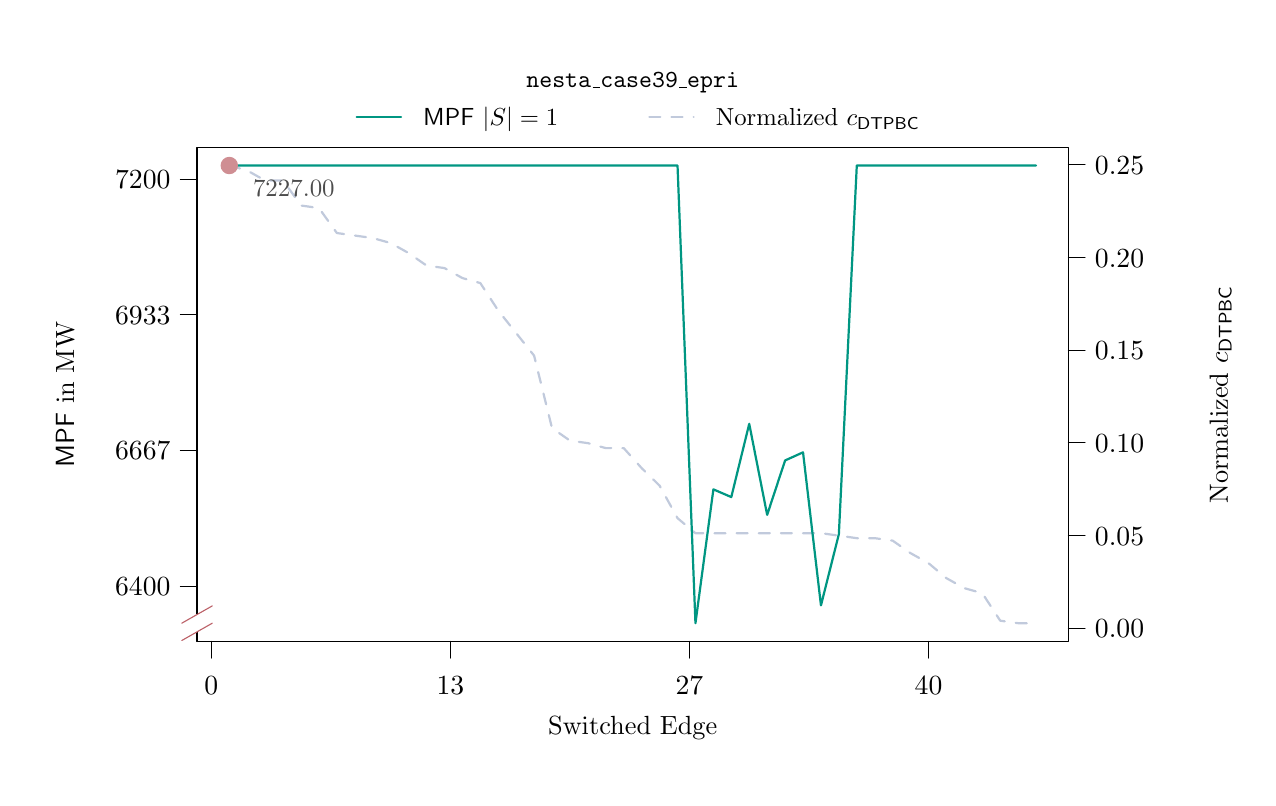
\begin{tikzpicture}[x=1pt,y=1pt]
\definecolor{fillColor}{RGB}{255,255,255}
\path[use as bounding box,fill=fillColor,fill opacity=0.00] (0,0) rectangle (440.85,271.01);
\begin{scope}
\path[clip] (  0.00,  0.00) rectangle (440.85,271.01);
\definecolor{drawColor}{RGB}{193,202,220}

\path[draw=drawColor,line width= 0.8pt,dash pattern=on 4pt off 4pt ,line join=round,line cap=round] ( 72.86,221.20) --
	( 79.34,219.39) --
	( 85.82,215.77) --
	( 92.30,215.77) --
	( 98.77,206.74) --
	(105.25,205.83) --
	(111.73,196.80) --
	(118.21,195.89) --
	(124.69,194.99) --
	(131.17,193.18) --
	(137.64,189.57) --
	(144.12,185.05) --
	(150.60,184.14) --
	(157.08,180.53) --
	(163.56,178.72) --
	(170.04,168.78) --
	(176.51,160.65) --
	(182.99,152.51) --
	(189.47,126.31) --
	(195.95,121.79) --
	(202.43,120.88) --
	(208.91,119.08) --
	(215.38,119.08) --
	(221.86,111.85) --
	(228.34,105.52) --
	(234.82, 93.77) --
	(241.30, 88.35) --
	(247.78, 88.35) --
	(254.25, 88.35) --
	(260.73, 88.35) --
	(267.21, 88.35) --
	(273.69, 88.35) --
	(280.17, 88.35) --
	(286.65, 88.35) --
	(293.12, 87.45) --
	(299.60, 86.54) --
	(306.08, 86.54) --
	(312.56, 85.64) --
	(319.04, 81.12) --
	(325.52, 77.50) --
	(331.99, 72.08) --
	(338.47, 68.47) --
	(344.95, 66.66) --
	(351.43, 56.72) --
	(357.91, 55.82) --
	(364.39, 55.82);
\end{scope}
\begin{scope}
\path[clip] (  0.00,  0.00) rectangle (440.85,271.01);
\definecolor{drawColor}{RGB}{0,0,0}

\path[draw=drawColor,line width= 0.4pt,line join=round,line cap=round] ( 61.20, 49.20) --
	(376.05, 49.20) --
	(376.05,227.81) --
	( 61.20,227.81) --
	( 61.20, 49.20);
\end{scope}
\begin{scope}
\path[clip] (  0.00,  0.00) rectangle (440.85,271.01);
\definecolor{drawColor}{RGB}{0,0,0}

\path[draw=drawColor,line width= 0.4pt,line join=round,line cap=round] (376.05, 54.01) -- (376.05,221.42);

\path[draw=drawColor,line width= 0.4pt,line join=round,line cap=round] (376.05, 54.01) -- (382.05, 54.01);

\path[draw=drawColor,line width= 0.4pt,line join=round,line cap=round] (376.05, 87.49) -- (382.05, 87.49);

\path[draw=drawColor,line width= 0.4pt,line join=round,line cap=round] (376.05,120.97) -- (382.05,120.97);

\path[draw=drawColor,line width= 0.4pt,line join=round,line cap=round] (376.05,154.46) -- (382.05,154.46);

\path[draw=drawColor,line width= 0.4pt,line join=round,line cap=round] (376.05,187.94) -- (382.05,187.94);

\path[draw=drawColor,line width= 0.4pt,line join=round,line cap=round] (376.05,221.42) -- (382.05,221.42);

\node[text=drawColor,anchor=base west,inner sep=0pt, outer sep=0pt, scale=  1.00] at (385.65, 50.56) {0.00};

\node[text=drawColor,anchor=base west,inner sep=0pt, outer sep=0pt, scale=  1.00] at (385.65, 84.05) {0.05};

\node[text=drawColor,anchor=base west,inner sep=0pt, outer sep=0pt, scale=  1.00] at (385.65,117.53) {0.10};

\node[text=drawColor,anchor=base west,inner sep=0pt, outer sep=0pt, scale=  1.00] at (385.65,151.01) {0.15};

\node[text=drawColor,anchor=base west,inner sep=0pt, outer sep=0pt, scale=  1.00] at (385.65,184.50) {0.20};

\node[text=drawColor,anchor=base west,inner sep=0pt, outer sep=0pt, scale=  1.00] at (385.65,217.98) {0.25};
\end{scope}
\begin{scope}
\path[clip] (  0.00,  0.00) rectangle (440.85,271.01);
\definecolor{drawColor}{RGB}{0,150,130}

\path[draw=drawColor,line width= 0.8pt,line join=round,line cap=round] (118.89,238.60) -- (134.91,238.60);
\definecolor{drawColor}{RGB}{193,202,220}

\path[draw=drawColor,line width= 0.8pt,dash pattern=on 4pt off 4pt ,line join=round,line cap=round] (224.63,238.60) -- (240.65,238.60);
\definecolor{drawColor}{RGB}{0,0,0}

\node[text=drawColor,anchor=base,inner sep=0pt, outer sep=0pt, scale=  0.89] at (218.62,249.28) {\texttt{nesta\_case39\_epri}};

\node[text=drawColor,anchor=base west,inner sep=0pt, outer sep=0pt, scale=  0.89] at (142.92,235.54) {$\mathsf{MPF}~|S|=1$};

\node[text=drawColor,anchor=base west,inner sep=0pt, outer sep=0pt, scale=  0.89] at (248.66,235.54) {Normalized~$c_\mathsf{DTPBC}$};
\end{scope}
\begin{scope}
\path[clip] (  0.00,  0.00) rectangle (440.85,271.01);
\definecolor{drawColor}{RGB}{0,0,0}

\path[draw=drawColor,line width= 0.4pt,line join=round,line cap=round] ( 61.20, 69.23) -- ( 61.20,216.24);

\path[draw=drawColor,line width= 0.4pt,line join=round,line cap=round] ( 61.20, 69.23) -- ( 55.20, 69.23);

\path[draw=drawColor,line width= 0.4pt,line join=round,line cap=round] ( 61.20,118.23) -- ( 55.20,118.23);

\path[draw=drawColor,line width= 0.4pt,line join=round,line cap=round] ( 61.20,167.23) -- ( 55.20,167.23);

\path[draw=drawColor,line width= 0.4pt,line join=round,line cap=round] ( 61.20,216.24) -- ( 55.20,216.24);

\node[text=drawColor,anchor=base east,inner sep=0pt, outer sep=0pt, scale=  1.00] at ( 51.60, 65.79) {6400};

\node[text=drawColor,anchor=base east,inner sep=0pt, outer sep=0pt, scale=  1.00] at ( 51.60,114.79) {6667};

\node[text=drawColor,anchor=base east,inner sep=0pt, outer sep=0pt, scale=  1.00] at ( 51.60,163.79) {6933};

\node[text=drawColor,anchor=base east,inner sep=0pt, outer sep=0pt, scale=  1.00] at ( 51.60,212.79) {7200};
\end{scope}
\begin{scope}
\path[clip] (  0.00,  0.00) rectangle (440.85,271.01);
\definecolor{drawColor}{RGB}{255,255,255}
\definecolor{fillColor}{RGB}{255,255,255}

\path[draw=drawColor,line width= 0.4pt,line join=round,line cap=round,fill=fillColor] ( 55.69, 52.69) rectangle ( 66.71, 58.94);
\definecolor{drawColor}{RGB}{188,97,104}

\path[draw=drawColor,line width= 0.4pt,line join=round,line cap=round] ( 55.69, 49.56) -- ( 66.71, 55.82);

\path[draw=drawColor,line width= 0.4pt,line join=round,line cap=round] ( 55.69, 55.82) -- ( 66.71, 62.07);
\end{scope}
\begin{scope}
\path[clip] ( 61.20, 49.20) rectangle (376.05,227.81);
\definecolor{drawColor}{RGB}{0,150,130}

\path[draw=drawColor,line width= 0.8pt,line join=round,line cap=round] ( 72.86,221.20) --
	( 79.34,221.20) --
	( 85.82,221.20) --
	( 92.30,221.20) --
	( 98.77,221.20) --
	(105.25,221.20) --
	(111.73,221.20) --
	(118.21,221.20) --
	(124.69,221.20) --
	(131.17,221.20) --
	(137.64,221.20) --
	(144.12,221.20) --
	(150.60,221.20) --
	(157.08,221.20) --
	(163.56,221.20) --
	(170.04,221.20) --
	(176.51,221.20) --
	(182.99,221.20) --
	(189.47,221.20) --
	(195.95,221.20) --
	(202.43,221.20) --
	(208.91,221.20) --
	(215.38,221.20) --
	(221.86,221.20) --
	(228.34,221.20) --
	(234.82,221.20) --
	(241.30, 55.82) --
	(247.78,104.18) --
	(254.25,101.39) --
	(260.73,127.85) --
	(267.21, 94.96) --
	(273.69,114.62) --
	(280.17,117.56) --
	(286.65, 62.25) --
	(293.12, 87.97) --
	(299.60,221.20) --
	(306.08,221.20) --
	(312.56,221.20) --
	(319.04,221.20) --
	(325.52,221.20) --
	(331.99,221.20) --
	(338.47,221.20) --
	(344.95,221.20) --
	(351.43,221.20) --
	(357.91,221.20) --
	(364.39,221.20);
\end{scope}
\begin{scope}
\path[clip] ( 61.20, 49.20) rectangle (376.05,227.81);
\definecolor{fillColor}{RGB}{207,142,147}

\path[fill=fillColor] ( 72.86,221.20) circle (  3.15);
\end{scope}
\begin{scope}
\path[clip] ( 61.20, 49.20) rectangle (376.05,227.81);
\definecolor{drawColor}{gray}{0.30}

\node[text=drawColor,anchor=base,inner sep=0pt, outer sep=0pt, scale=  0.90] at ( 96.18,210.04) {7227.00};
\end{scope}
\begin{scope}
\path[clip] (  0.00,  0.00) rectangle (440.85,271.01);
\definecolor{drawColor}{RGB}{0,0,0}

\path[draw=drawColor,line width= 0.4pt,line join=round,line cap=round] ( 66.38, 49.20) -- (325.52, 49.20);

\path[draw=drawColor,line width= 0.4pt,line join=round,line cap=round] ( 66.38, 49.20) -- ( 66.38, 43.20);

\path[draw=drawColor,line width= 0.4pt,line join=round,line cap=round] (152.76, 49.20) -- (152.76, 43.20);

\path[draw=drawColor,line width= 0.4pt,line join=round,line cap=round] (239.14, 49.20) -- (239.14, 43.20);

\path[draw=drawColor,line width= 0.4pt,line join=round,line cap=round] (325.52, 49.20) -- (325.52, 43.20);

\node[text=drawColor,anchor=base,inner sep=0pt, outer sep=0pt, scale=  1.00] at ( 66.38, 30.00) {0};

\node[text=drawColor,anchor=base,inner sep=0pt, outer sep=0pt, scale=  1.00] at (152.76, 30.00) {13};

\node[text=drawColor,anchor=base,inner sep=0pt, outer sep=0pt, scale=  1.00] at (239.14, 30.00) {27};

\node[text=drawColor,anchor=base,inner sep=0pt, outer sep=0pt, scale=  1.00] at (325.52, 30.00) {40};

\node[text=drawColor,anchor=base,inner sep=0pt, outer sep=0pt, scale=  0.95] at (218.62, 15.60) {Switched Edge};

\node[text=drawColor,rotate= 90.00,anchor=base,inner sep=0pt, outer sep=0pt, scale=  0.95] at ( 16.80,138.51) {$\mathsf{MPF}$ in~$\mathrm{MW}$};

\node[text=drawColor,rotate= 90.00,anchor=base,inner sep=0pt, outer sep=0pt, scale=  0.95] at (433.65,138.51) {Normalized~$c_\mathsf{DTPBC}$};
\end{scope}
\end{tikzpicture}
